\documentclass[a4paper]{article}
\usepackage{latexsym}
\usepackage[a4paper]{geometry}
\usepackage{color}
\usepackage{listings}
\usepackage[pdftex]{graphicx}
\usepackage{float}
\usepackage{mathtools}
\usepackage{amsfonts, amsthm, amssymb}

\definecolor{Blue}{rgb}{0,0,0.5}
\definecolor{Green}{rgb}{0,0.75,0.0}
\definecolor{LightGray}{rgb}{0.6,0.6,0.6}
\definecolor{DarkGray}{rgb}{0.3,0.3,0.3}
\lstset{language=Matlab,
   keywords={function,uint8,uint16,uint32,double,break,case,catch,continue,else,elseif,end,for,global,if,otherwise,persistent,return,switch,try,while},
   basicstyle=\ttfamily\small,
   breaklines=true,
   keywordstyle=\bfseries\color{Blue},
   commentstyle=\itshape\color{LightGray},
   stringstyle=\color{Green},
   numbers=left,
   numberstyle=\tiny\color{DarkGray},
   stepnumber=1,
   numbersep=10pt,
   backgroundcolor=\color{white},
   tabsize=2,
   showspaces=false,
   showstringspaces=false,
   captionpos=b}

%Boldface text for type writer font
\usepackage{bold-extra} %\DeclareFontShape{OT1}{cmtt}{bx}{n}{<5><6><7><8><9><10><10.95><12><14.4><17.28><20.74><24.88>cmttb10}{}

%Break words properly at the end of a line (which isn't sloppy...)
\sloppy

%Use command \exercise for each exercise
\newcounter{exerciseCount}
\setcounter{exerciseCount}{0}
\newcommand{\exercise}[1]{\addtocounter{exerciseCount}{1} \noindent \medskip {\large \textsf{\textbf{Exercise \arabic{exerciseCount} \--- #1}}} \par}
\renewcommand{\theenumi}{\textsf{\textbf{\alph{enumi}}}}

%Use command \code for code snippets
\newcommand{\code}[1]{\textnormal{\texttt{#1}}}

\newtheorem*{claim}{Claim}
\renewcommand\qedsymbol{$\blacksquare$}

\title{\textsf{Image Processing \\ lab 4}}
\author{Klaas Kliffen \and Jan Kramer}
\date{\today}

\begin{document}
\maketitle

\exercise{Skeletons}
\noindent
The morphological skeleton of an image X with structuring element B is defined as:
\[
    SK(X) = \bigcup_{k = 0}^K S_{k}(X)
\]
where
\[
    S_{k}(X) = (X\ominus kB) - (X \ominus kB) \circ B
\]
and $K \in \mathbb{N}$ such that
\[
    K = max\{k |(X\ominus kB) \neq \emptyset\}.
\]
In addition $(X\ominus kB)$ is defined as follows:
\[
    (X \ominus kB) =
         \begin{cases}
             X      & \quad \text{if } k = 0\\
             ((\dots(X \ominus B) \ominus B) \ominus \dots) \ominus B) & \quad \text{otherwise} \\
         \end{cases}
\]
Note that in the second case $\ominus B$ is applied $k$ times to $X$.
\begin{enumerate}
\item
Let set $B = \hat{B} = \{0\}$ be given. \\
\begin{claim}
    $SK(X) = \emptyset$
\end{claim}
\begin{proof}
Note that for all $z \in \mathbb{Z}^{2}$ the following holds:
\[
    (B)_{z} = \{c|c = b + z, b \in B\} = \{c|c = z\} = \{z\}
\]
Then we have by the definition of the erosion of $X$ by $B$ that
\begin{align} \label{eq:ominus}
    X \ominus B &= \{z | (B)_{z} \subseteq X\} \nonumber\\
                &= \{z | \{z\} \subseteq X\} \\
                &= X. \nonumber
\end{align}
Similarly we have by the definition of the dilution of $X$ by $B$ that
\begin{align} \label{eq:oplus}
    X \oplus B &= \{z | (\hat{B})_{z} \cap X \neq \emptyset\} \nonumber\\
               &= \{z | \{z\} \cap X \neq \emptyset\} \\
               &= X. \nonumber
\end{align}
The skeleton of image $X$ with structuring element $B$ is:
\begin{align*}
    SK(X) &= \bigcup_{k = 0}^K S_{k}(X) \\
          &= \bigcup_{k = 0}^K \left((X\ominus kB) - (X \ominus kB) \circ B\right) \\
          &= \bigcup_{k = 0}^K \left((X \ominus kB) - ((X \ominus kB) \ominus B) \oplus B\right) \\
\end{align*}
Now if we apply the definition of $(X \ominus kB)$ and the results of equation \ref{eq:ominus} and \ref{eq:oplus} we get:
\begin{align*}
    SK(X) &= \bigcup_{k = 0}^K \left((X \ominus kB) - ((X \ominus kB) \ominus B) \oplus B\right) \\
          &= \bigcup_{k = 0}^K \left(X - X\right) \\
          &= \bigcup_{k = 0}^K \emptyset \\
          &= \emptyset
\end{align*}
\end{proof}

\item 
Let $X \ominus B = \emptyset$ be given.
\begin{claim}
    SK(X) = X
\end{claim}
\begin{proof}
Consider the definition of $(X \ominus kB)$:
\[
    (X \ominus kB) =
         \begin{cases}
             X      & \quad \text{if } k = 0\\
             ((\dots(X \ominus B) \ominus B) \ominus \dots) \ominus B) & \quad \text{otherwise} \\
         \end{cases}
\]
Note that $X \ominus B = \emptyset$. In addition for $X = \emptyset$ we have that every other erosion in the definition above is
\begin{equation} \label{eq:eominus}
    X \ominus B = \emptyset \ominus B = \{z | (B)_{z} \subseteq \emptyset\} = \emptyset.
\end{equation}
Hence the previous definition $X \ominus kB$ is equal to:
\begin{equation} \label{eq:kB}
    (X \ominus kB) =
         \begin{cases}
             X      & \quad \text{if } k = 0\\
             \emptyset & \quad \text{otherwise} \\
         \end{cases}
\end{equation}
Now the skeleton of image $X$ with structuring element $B$ is:
\begin{align*}
    SK(X) &= \bigcup_{k = 0}^K S_{k}(X) \\
          &= \bigcup_{k = 0}^K \left((X\ominus kB) - (X \ominus kB) \circ B\right) \\
          &= \bigcup_{k = 0}^K \left((X \ominus kB) - ((X \ominus kB) \ominus B) \oplus B\right) \\
          &= \left((X \ominus 0B) - ((X \ominus 0B) \ominus B) \oplus B\right) \cup \bigcup_{k = 1}^K \left((X \ominus kB) - ((X \ominus kB) \ominus B) \oplus B\right) \\
\end{align*}
If we use the equation \ref{eq:eominus}, \ref{eq:kB} and the definition of $X \oplus B$ we get:
\begin{align*}
    SK(X) &= \left(X - (X \ominus B) \oplus B\right) \cup \bigcup_{k = 1}^K \left(\emptyset - (\emptyset \ominus B) \oplus B\right) \\
          &= \left(X - (\emptyset \oplus B)\right) \cup \bigcup_{k = 1}^K \left(\emptyset - (\emptyset \oplus B)\right) \\
          &= \left(X - \{z | (\hat{B})_{z} \cap \emptyset \neq \emptyset\}\right) \cup \bigcup_{k = 1}^K \left(\emptyset - \{z | (\hat{B})_{z} \cap \emptyset \neq \emptyset\}\right) \\
          &= \left(X - \{z | \emptyset \neq \emptyset\}\right) \cup \bigcup_{k = 1}^K \left(\emptyset - \{z | \emptyset \neq \emptyset\}\right) \\
          &= \left(X - \emptyset \right) \cup \bigcup_{k = 1}^K \left(\emptyset - \emptyset\right) \\
          &= X \cup \bigcup_{k = 1}^K \emptyset \\
          &= X \cup \emptyset \\
          &= X 
\end{align*}
\end{proof}
\item
\lstinputlisting{../lab4ex1/IPdilate.m}
\lstinputlisting{../lab4ex1/IPerode.m}
\lstinputlisting{../lab4ex1/IPskeletondecomp.m}
\item
\lstinputlisting{../lab4ex1/IPskeletonrecon.m}
\item
\lstinputlisting{../lab4ex1/runex1.m}
The result of running this script is as follows:
\begin{lstlisting}
ans = 0.
\end{lstlisting}
This means that the origional and the resulting image are identical.
In addition these images can be seen in Figure \ref{fig:nutsbolts}.
\begin{figure}[H]
\centering
\begin{tabular}{ccc}
    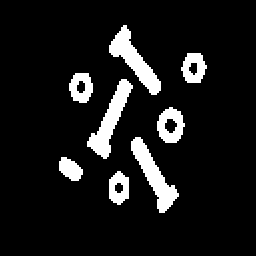
\includegraphics[width=0.3\textwidth]{../lab4ex1/nutsbolts.png} & 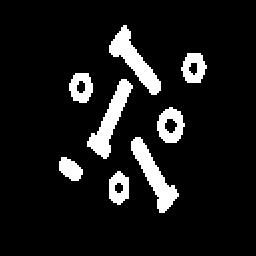
\includegraphics[width=0.3\textwidth]{../lab4ex1/recon.png}  & \\
    Original image & the result of the skeleton decomposition and reconstruction \\
\end{tabular}
\caption{The nutsbolts image and its skeleton decomposition reconstruction.}
\label{fig:nutsbolts}
\end{figure}
\end{enumerate}


\exercise{Grey-scale morphology}
\begin{enumerate}
\item
%\lstinputlisting{../lab3ex2/IPdwt2.m}
\item
%\begin{figure}[H]
%\centering
%\begin{tabular}{ccc}
%    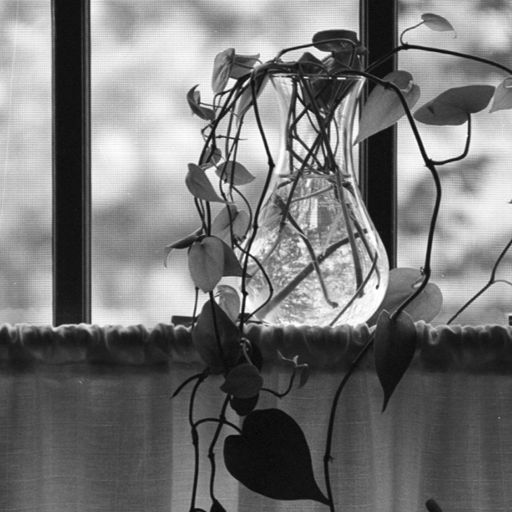
\includegraphics[width=0.3\textwidth]{../lab3ex2/vase.png} & 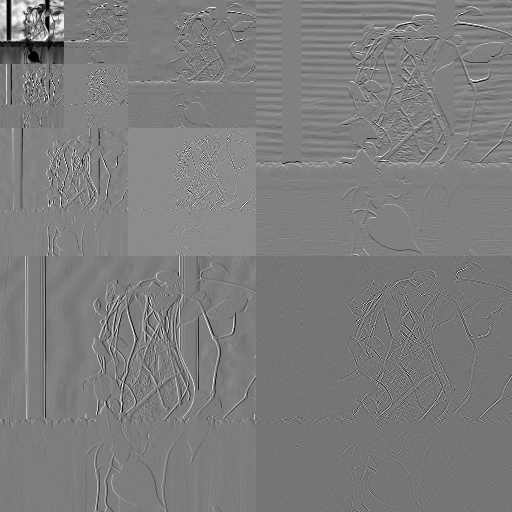
\includegraphics[width=0.3\textwidth]{../lab3ex2/scaled.png}  & \\
%    Original image & 3 scale wavelet transform & the layout labels of the transform \\
%\end{tabular}
%\caption{3 scale wavelet transform of the orignal image}
%\label{fig:wavelet}
%\end{figure}

\end{enumerate}

\exercise{Classification}

\newpage
\section*{Task distribution}

\begin{table}[H]
\centering
\begin{tabular}{ccccc}
ex1 & design & implementation & answers questions & writing report \\
\hline
Klaas & 60\% & 90\% & n.a. & 50\% \\
\hline
Jan & 40\% & 10\% & n.a. & 50\% \\
\end{tabular}
\end{table}

\begin{table}[H]
\centering
\begin{tabular}{ccccc}
ex2 & design & implementation & answers questions & writing report \\
\hline
Klaas & 50\% & 30\% & 25\% & 25\% \\
\hline
Jan & 50\% & 70\% & 75\% & 75\% \\
\end{tabular}
\end{table}

\begin{table}[H]
\centering
\begin{tabular}{ccccc}
ex3 & design & implementation & answers questions & writing report \\
\hline
Klaas & 50\% & 75\% & 50\% & 75\% \\
\hline
Jan & 50\% & 25\% & 50\% & 25\% \\
\end{tabular}
\end{table} 



\end{document}
